\chapter*{Glossar}\label{Glossar}
\markboth{Glossar}{}
\addcontentsline{toc}{chapter}{Glossar}
\begin{description}
  \item[Android] \hfill \\
    Android ist ein Betriebssystem von Google für mobile Geräte
  \item[Apache-Webserver] \hfill \\
    Ein Apache-Webserver ist ein Serverprogramm zum Ausliefern von Webseiten
  \item[Apple iOS] \hfill \\
    Apple iOS ist ein Betriebssystem von Apple für mobile Geräte
  \item[Backend] \hfill \\
    Backend ist der Teil einer Webseite, den Benutzer erst nach Anmeldung sehen können
  \item[Bluetooth] \hfill \\
    Bluetooth ist ein Protokoll zur kabellosen Übertragung von Daten über kurze Distanzen
  \item[Entity Relationship Diagramm] \hfill \\
    Ein Entity Relationship Diagram ist ein Diagramm zur Modellierung und Strukturierung von Beziehungen zwischen Datenbankentitäten
  \item[Framework] \hfill \\
    Ein Framework (dt.: Rahmenstruktur) ist ein Programmgerüst zur Bereitstellung von Rahmenfunktionen einer Anwendung
  \item[Frontend] \hfill \\
    Frontend ist der Teil einer Webseite, den Benutzer direkt sehen können
  \item[Header] \hfill \\
    Ein Header ist eine Zeile, die in der oberen Region einer Webseite zu finden ist
  \item[HTML] \hfill \\
    HTML ist eine Auszeichnungssprache zur Darstellung digitaler Dokumente
  \item[Java] \hfill \\
    Java ist eine objektorientierte Programmiersprache
  \item[Javascript] \hfill \\
    Javascript ist eine Programmiersprache zur Erweiterung von HTML und CSS
  \item[MMS] \hfill \\
    MMS (Multimedia Messaging Service) ist ein Dienst zum Austausch von multimedialen Nachrichten
  \item[Open Source] \hfill \\
    Open Source ist ein Entwicklungsmodell zur kostenfreien Lizenzierung und freien Verfügbarkeit des Programmcodes
  \item[Post-It] \hfill \\
    Post-It ist ein Markenname für Haftnotizen
  \item[Sidebar] \hfill \\
    Eine Sidebar ist ein seitliches Menü zur Bereitstellung von Funktionen
  \item[SMS] \hfill \\
    SMS (Short Message Service) ist ein Dienst zum Austausch von Textnachrichten
  \item[SMS Gateway] \hfill \\
    Ein SMS Gateway ist eine Schnittstelle zum Senden und Empfangen von SMS-Textnachrichten
  \item[Swipe] \hfill \\
    Swipe ist eine Geste zum Interagieren mit Touch-Oberflächen, bei der Nutzer mit ihren Fingern auf der Oberfläche in eine Richtung wischen
  \item[Tablet PC] \hfill \\
    Ein Tablet PC ist ein flacher kompakter Computer mit Touchscreen
  \item[Touchscreen] \hfill \\
    Ein Touchscreen ist ein Bildschirm mit sensibler Oberfläche zur Eingabe von Benutzeraktionen
  \item[UI] \hfill \\
    Ein UI (User Interface) ist ein Benutzerinterface zur Interaktion zwischen Benutzern und System
\end{description}

\chapter*{Anhang}\label{Anhang}
\markboth{Anhang - Paper Prototype}{}
\addcontentsline{toc}{chapter}{Anhang}
% \todotext{Scans}
\begin{figure}[h!]
  \centering
    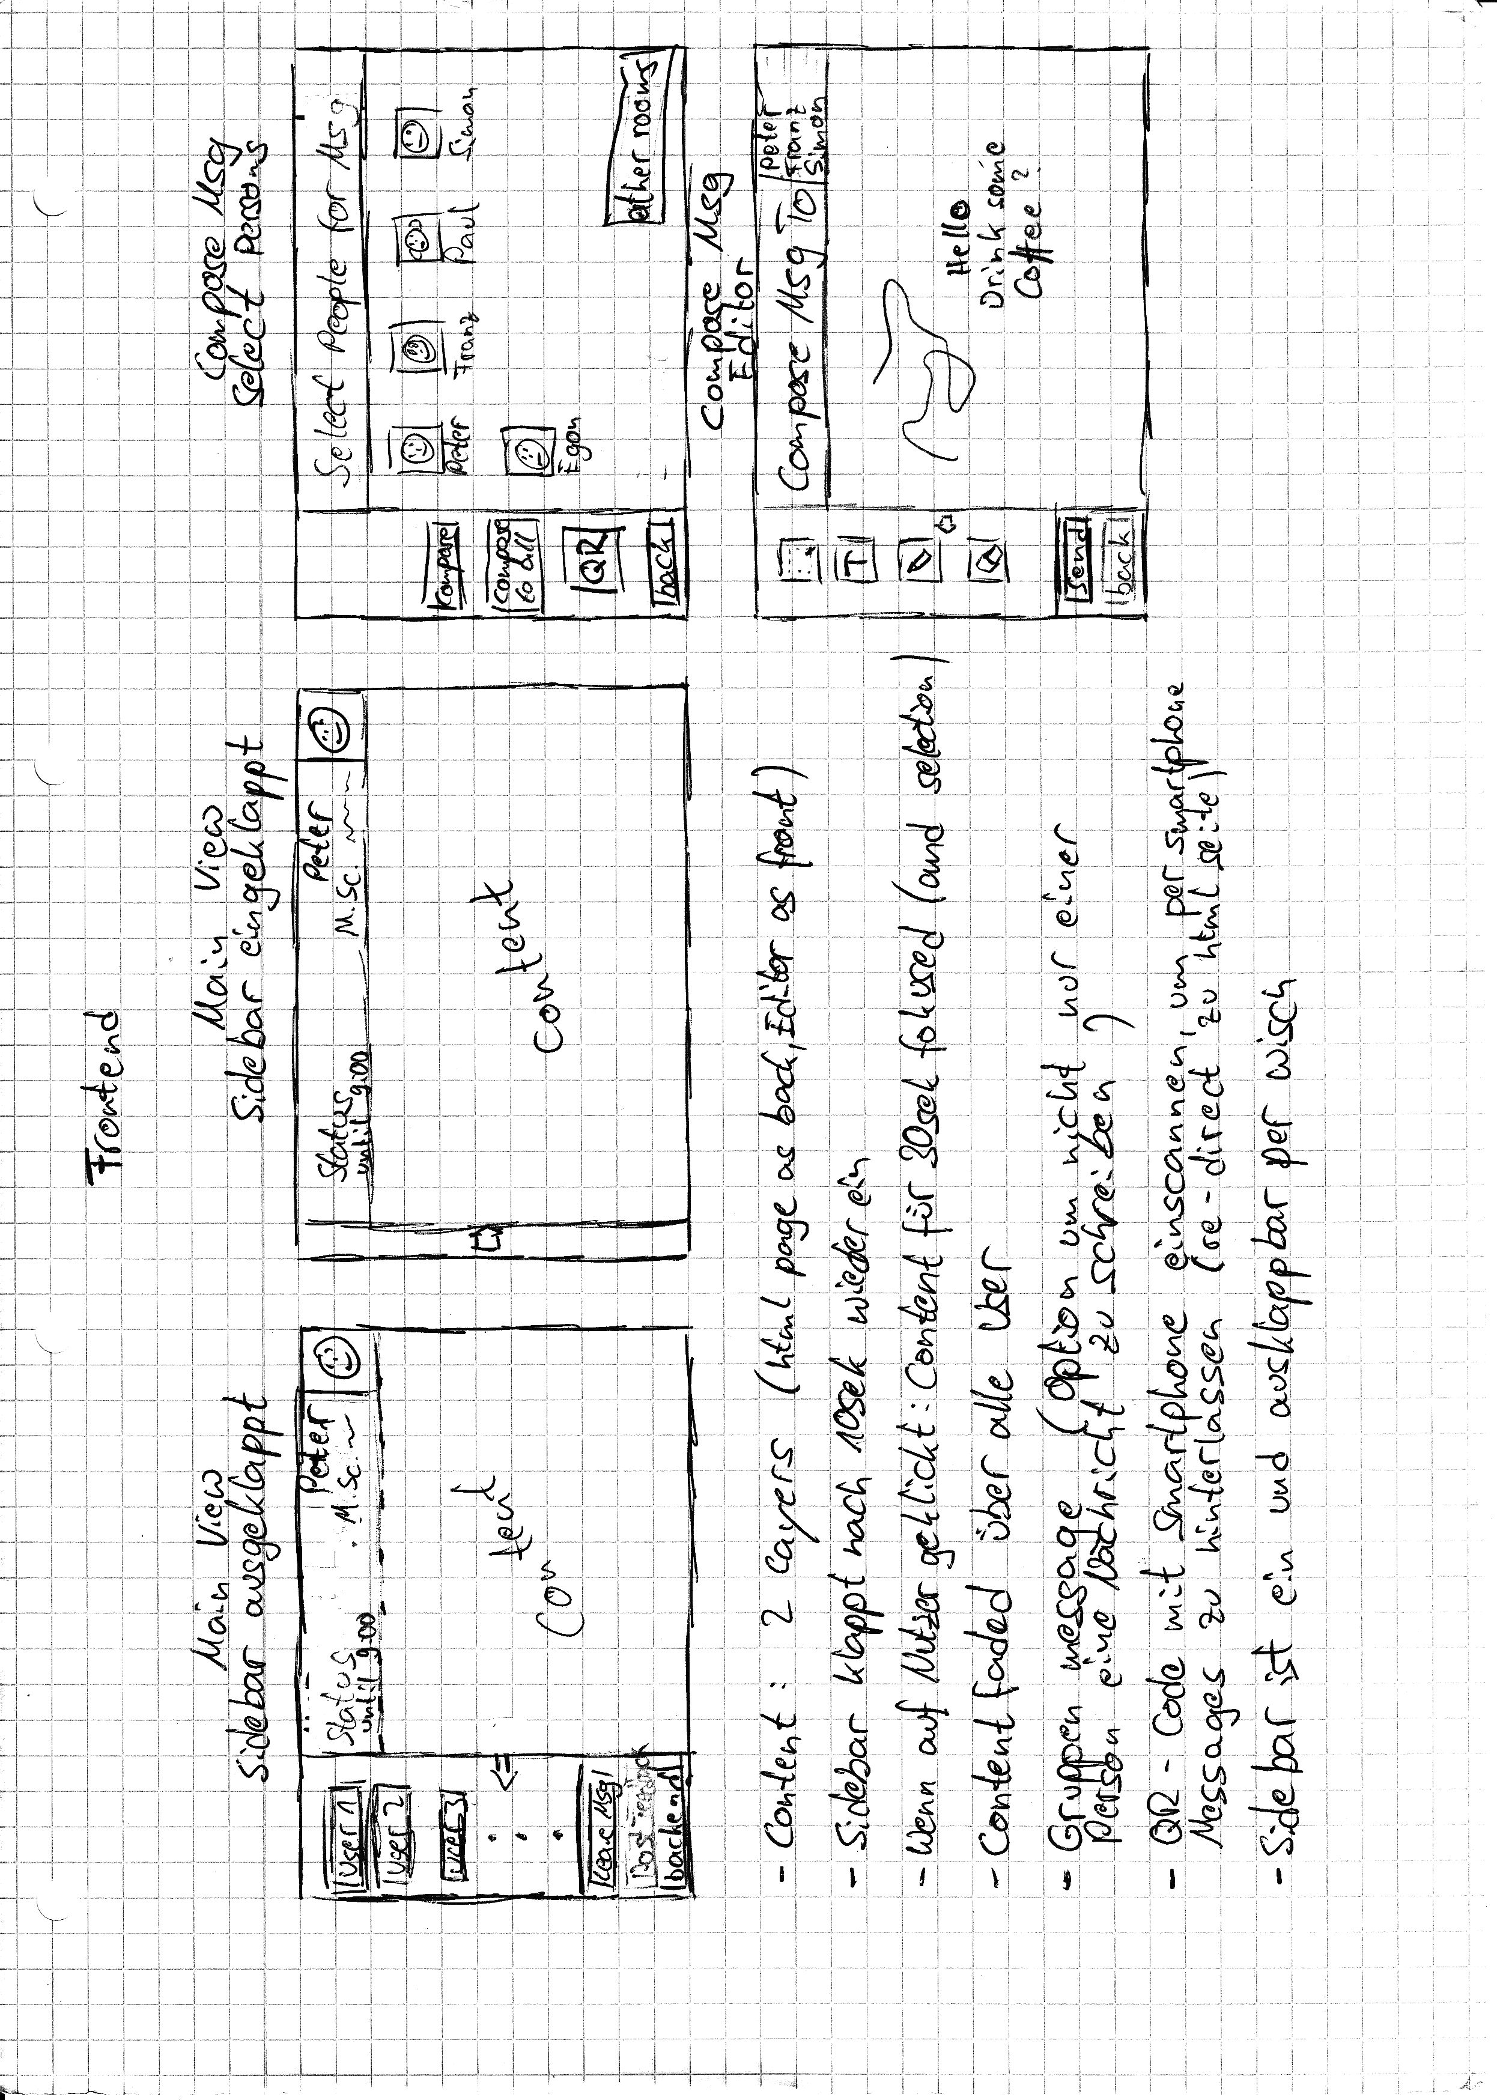
\includegraphics[width=0.75\textwidth]{./img/paperPrototype1.png}
  \caption{Paper Prototype - Frontend}
  \label{img:paperPrototypeFrontend}
\end{figure}

\newpage
\begin{figure}[h!]
  \centering
    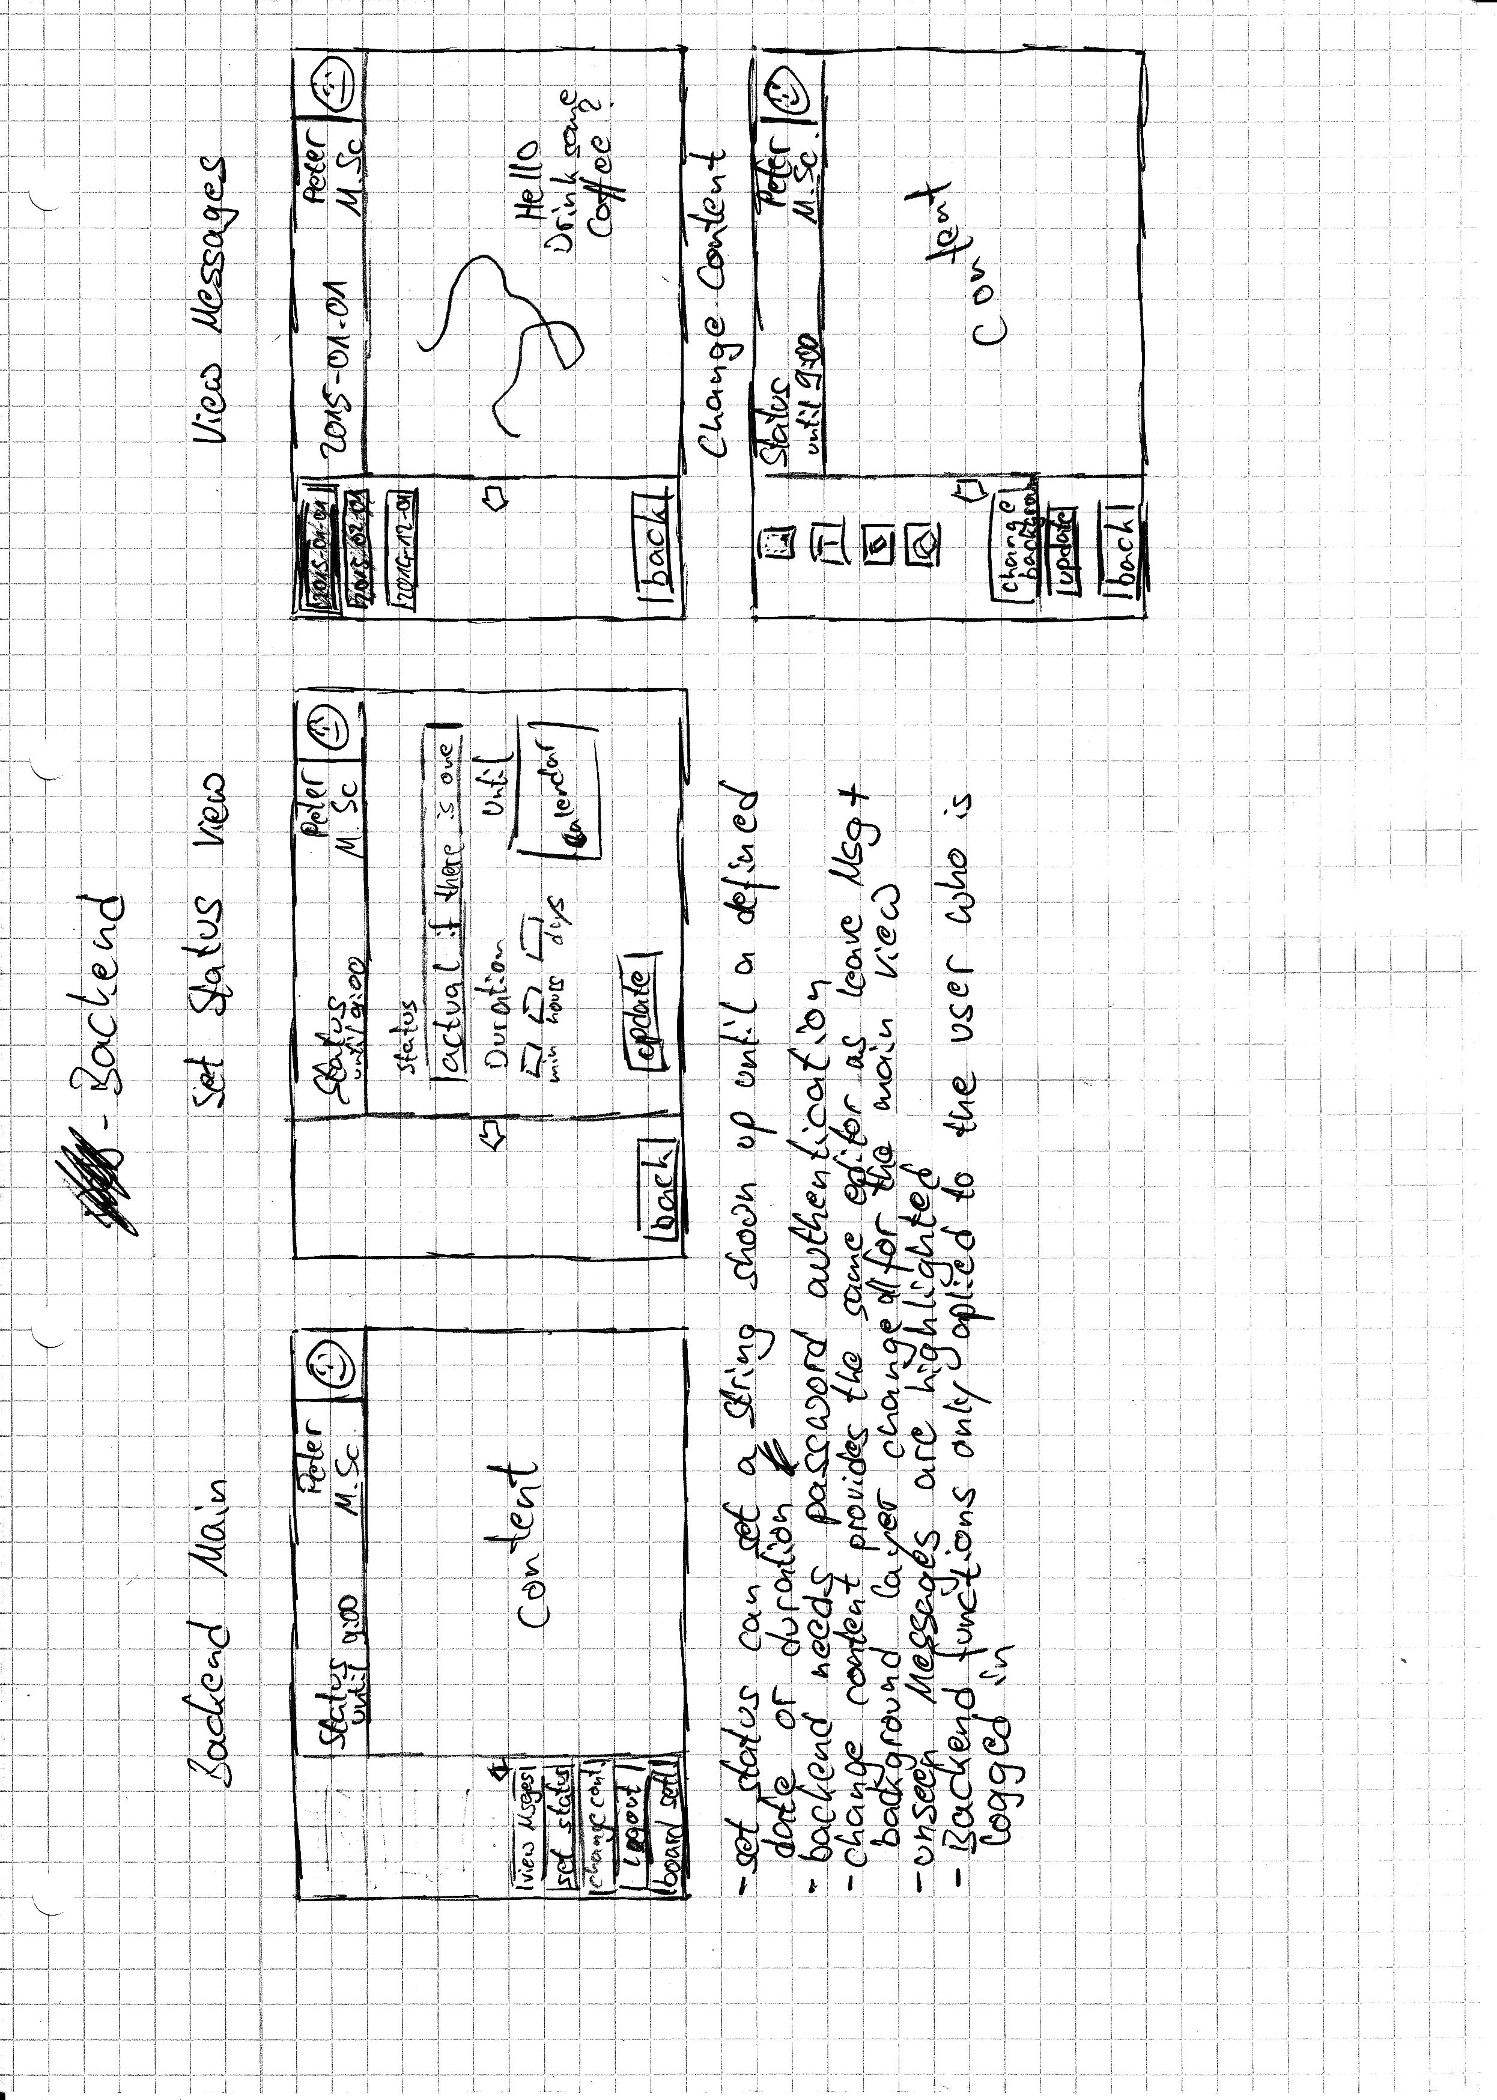
\includegraphics[width=1\textwidth]{./img/paperPrototypeBackend1.png}
  \caption{Paper Prototype - User Backend}
  \label{img:paperPrototypeBackend1}
\end{figure}

\newpage
\begin{figure}[h!]
  \centering
    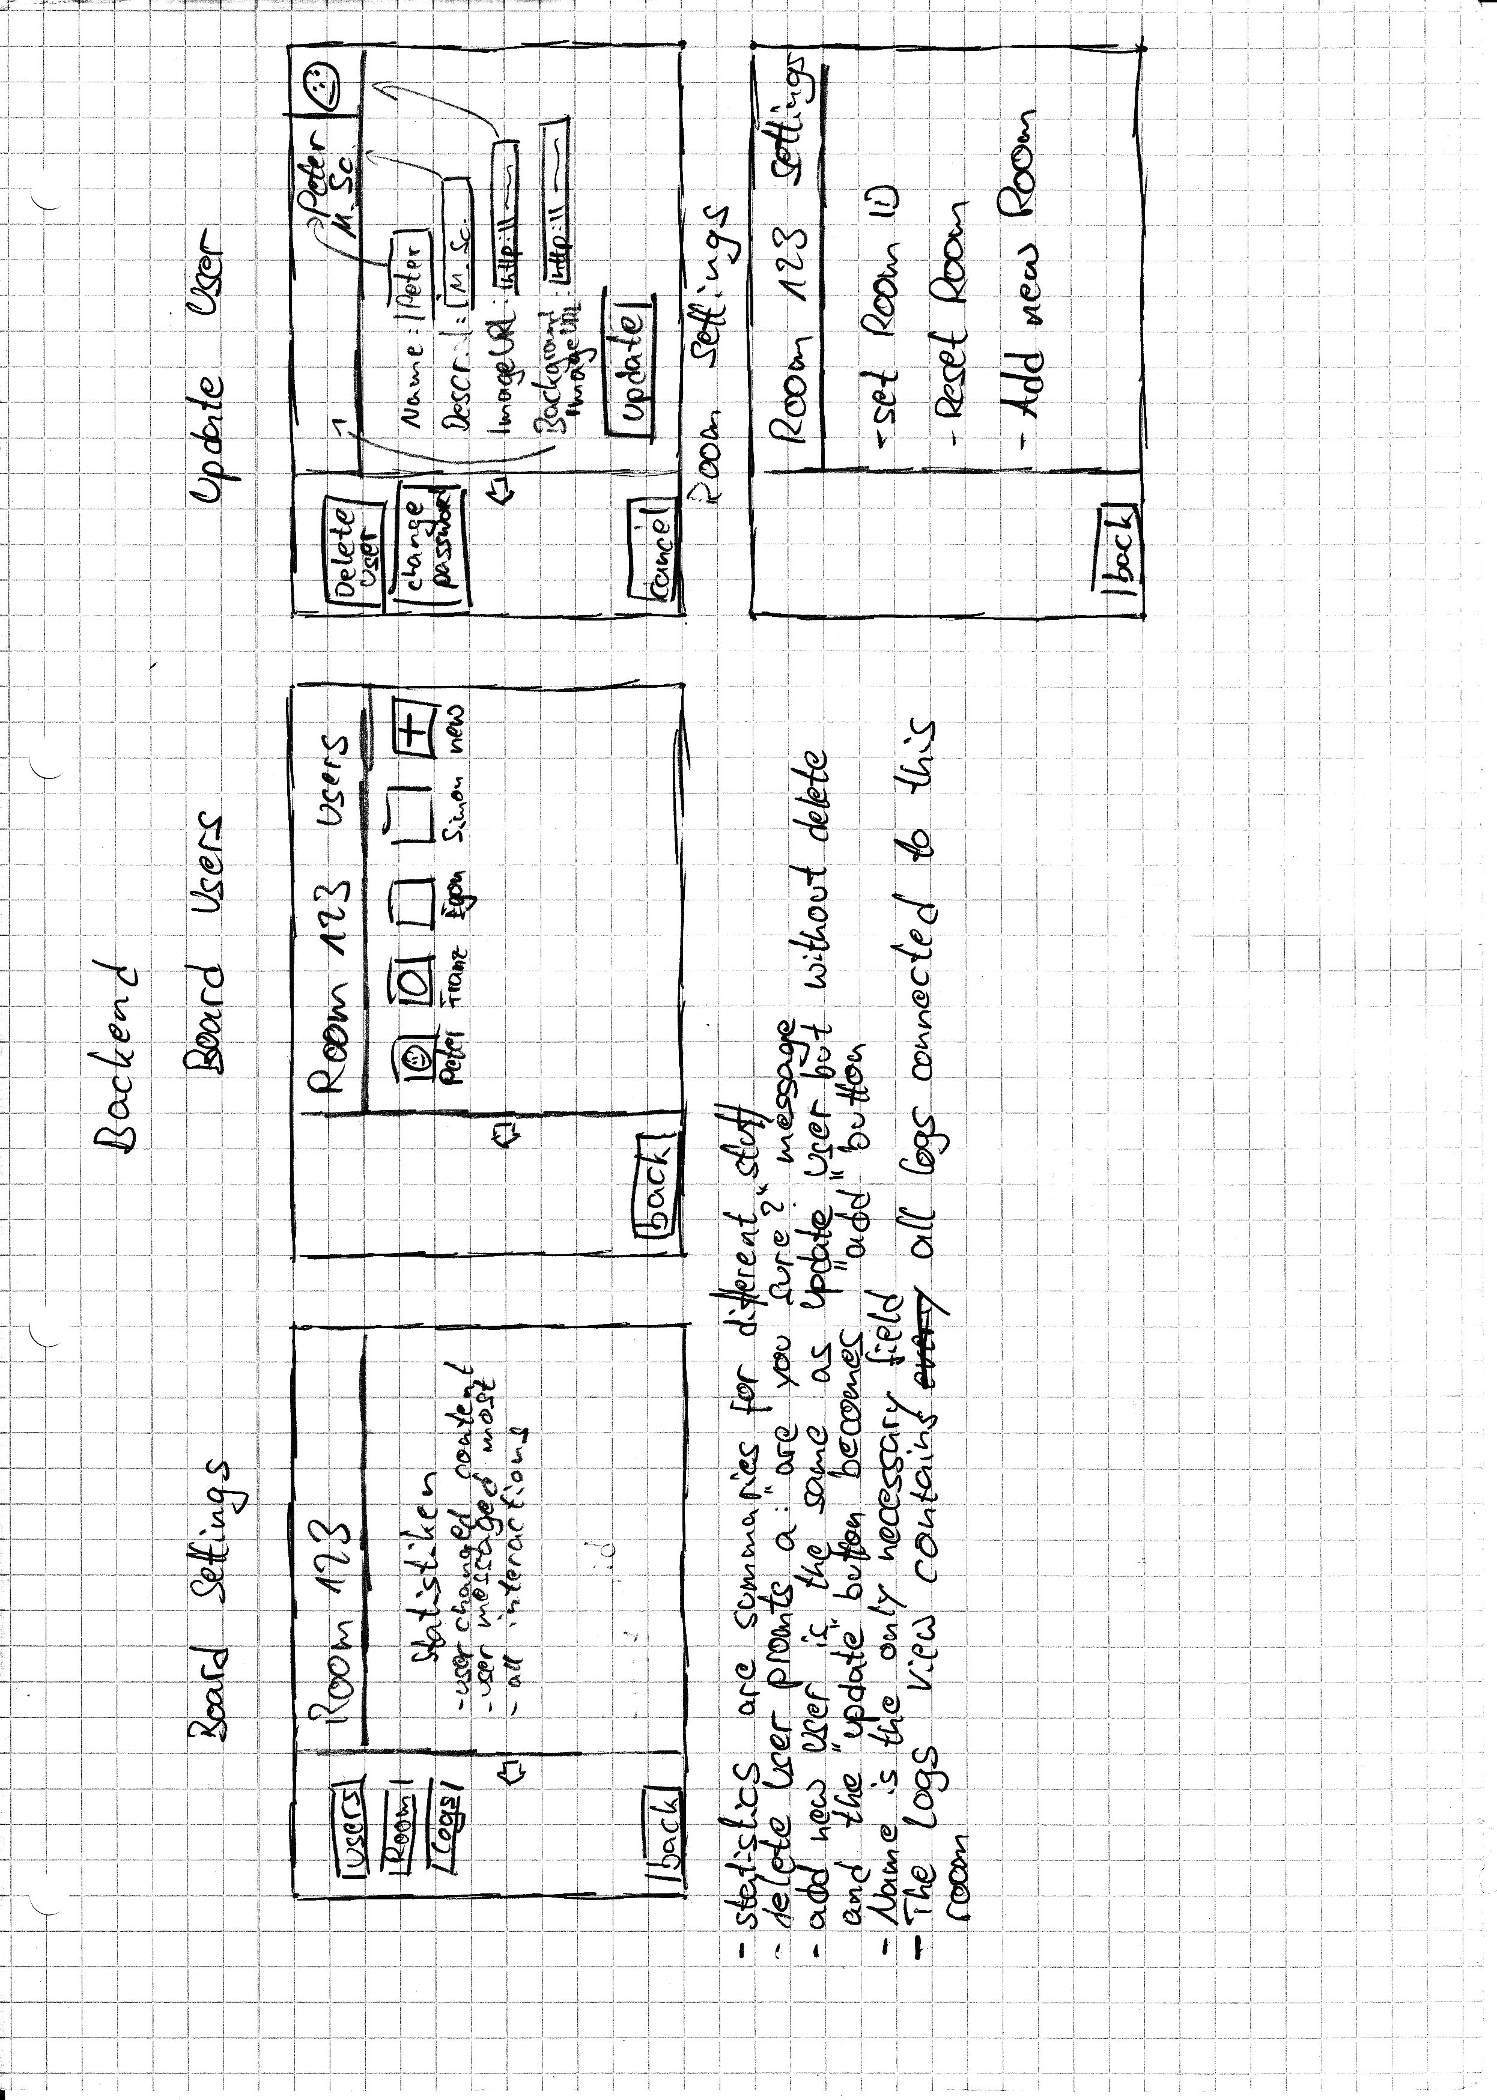
\includegraphics[width=1\textwidth]{./img/paperPrototypeBackend2.png}
  \caption{Paper Prototype - Admin Backend}
  \label{img:paperPrototypeBackend2}
\end{figure}
\newpage
\begin{figure}[h!]
  \centering
    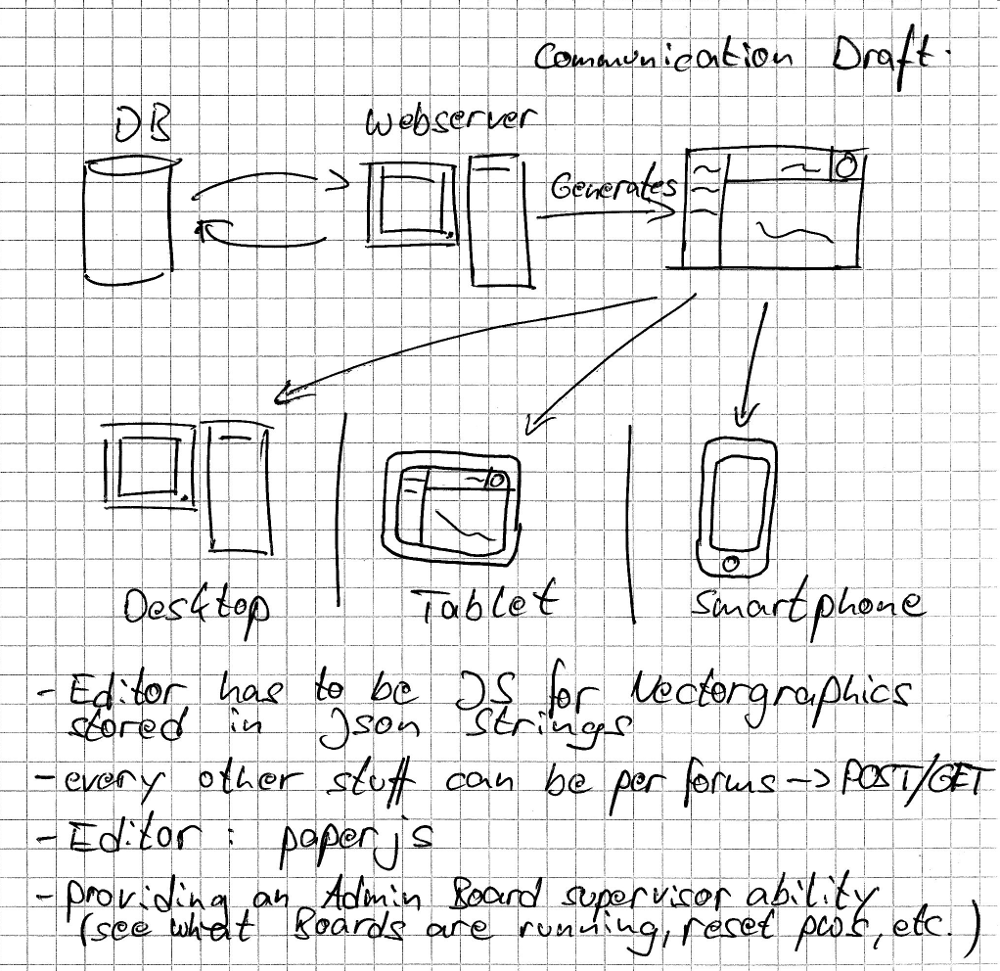
\includegraphics[width=0.8\textwidth]{./img/draftCommunication.png}
  \caption{Entwurf - Systemaufbau}
  \label{img:anhangLocations}
\end{figure}
\begin{figure}[h!]
  \centering
    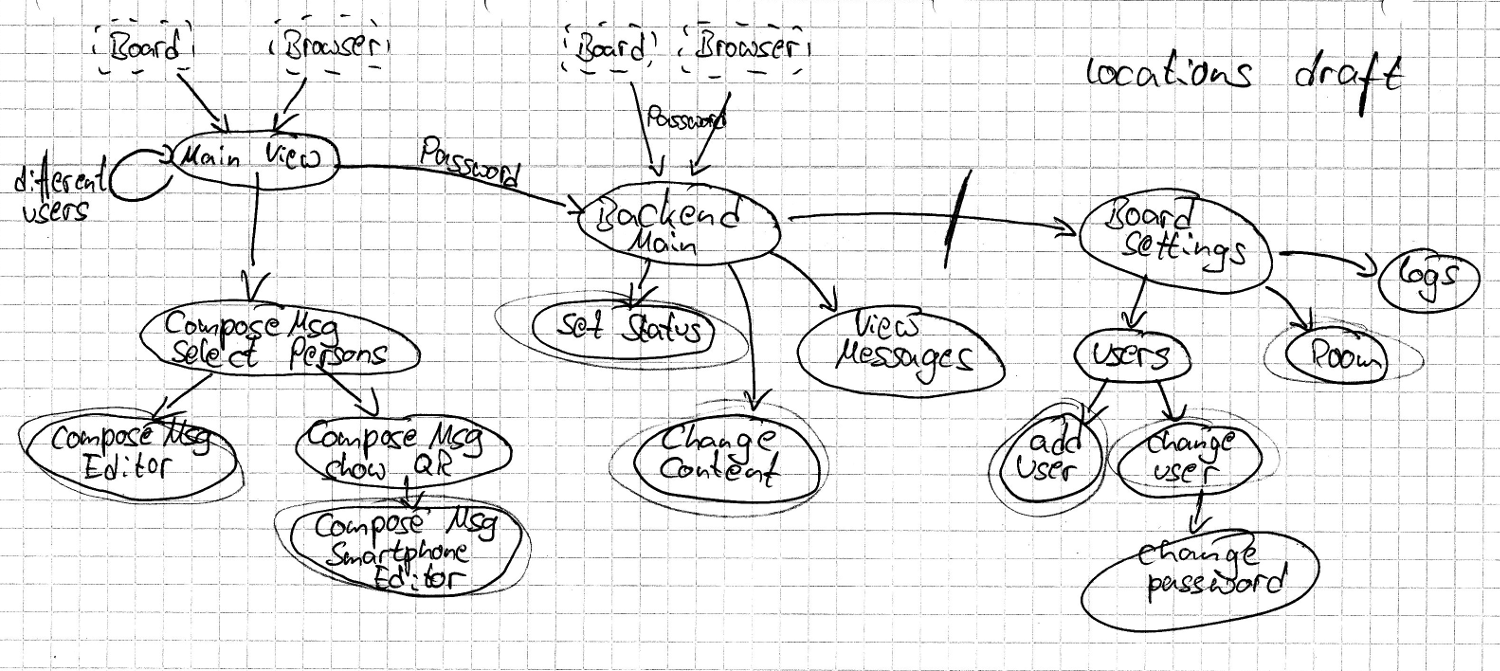
\includegraphics[width=1\textwidth]{./img/draftLocations.png}
  \caption{Entwurf - Funktionen}
  \label{img:anhangFunktionen}
\end{figure}
\newpage
\begin{figure}[h!]
  \centering
    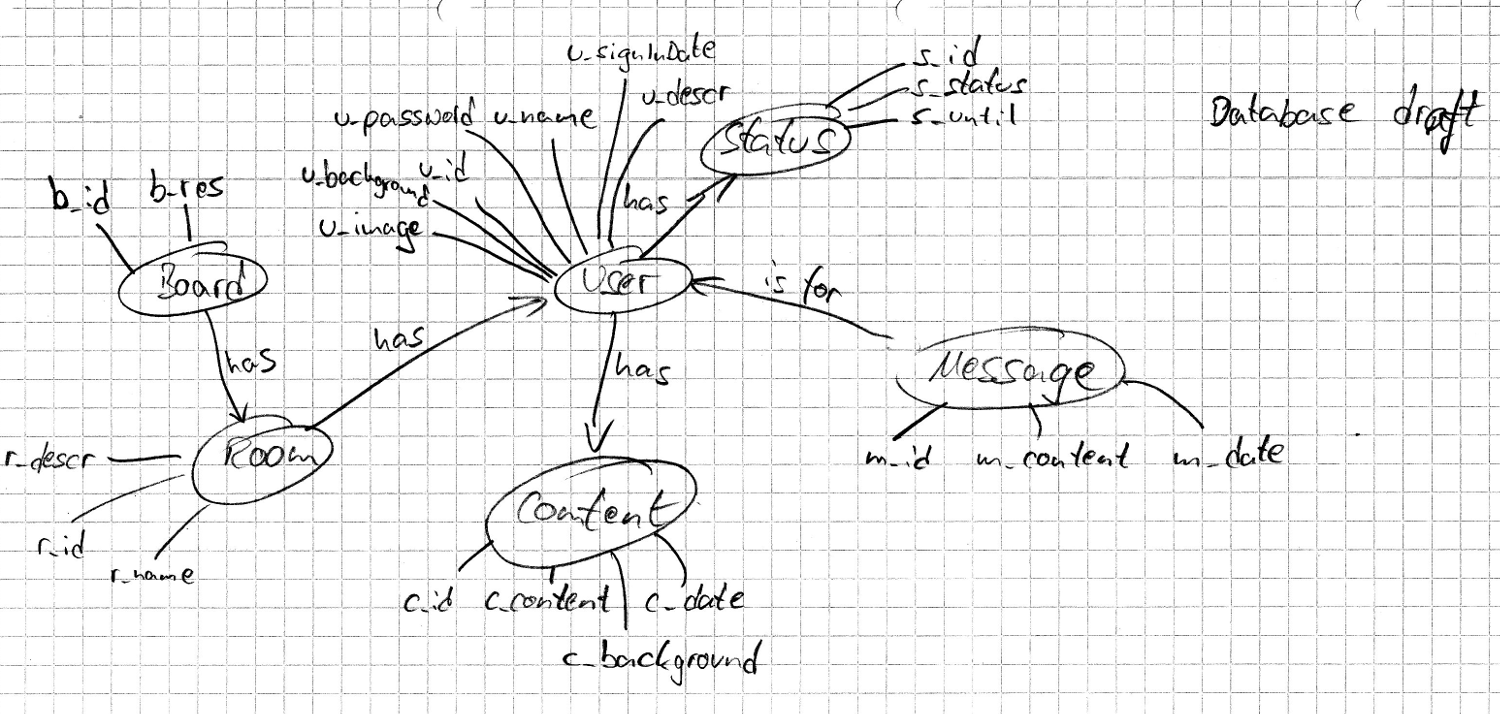
\includegraphics[width=1\textwidth]{./img/draftDatabase.png}
  \caption{Entwurf - Datenbank}
  \label{img:anhangDatenbank}
\end{figure}
\newpage
%%%%%%%%%%%%%%%%%%%%%%%%%%%%%%%%%%%%%%%%%%%%%%%%%%%%%%%%%%%%%%%%%%%%%%%%%%%%%%%%%%%%%%%%%%%%%%%%%%%%%%%%%%%%%%%%
\markboth{Anhang - Benutzerhandbuch}{}
\begin{figure}[h!]
  \centering
    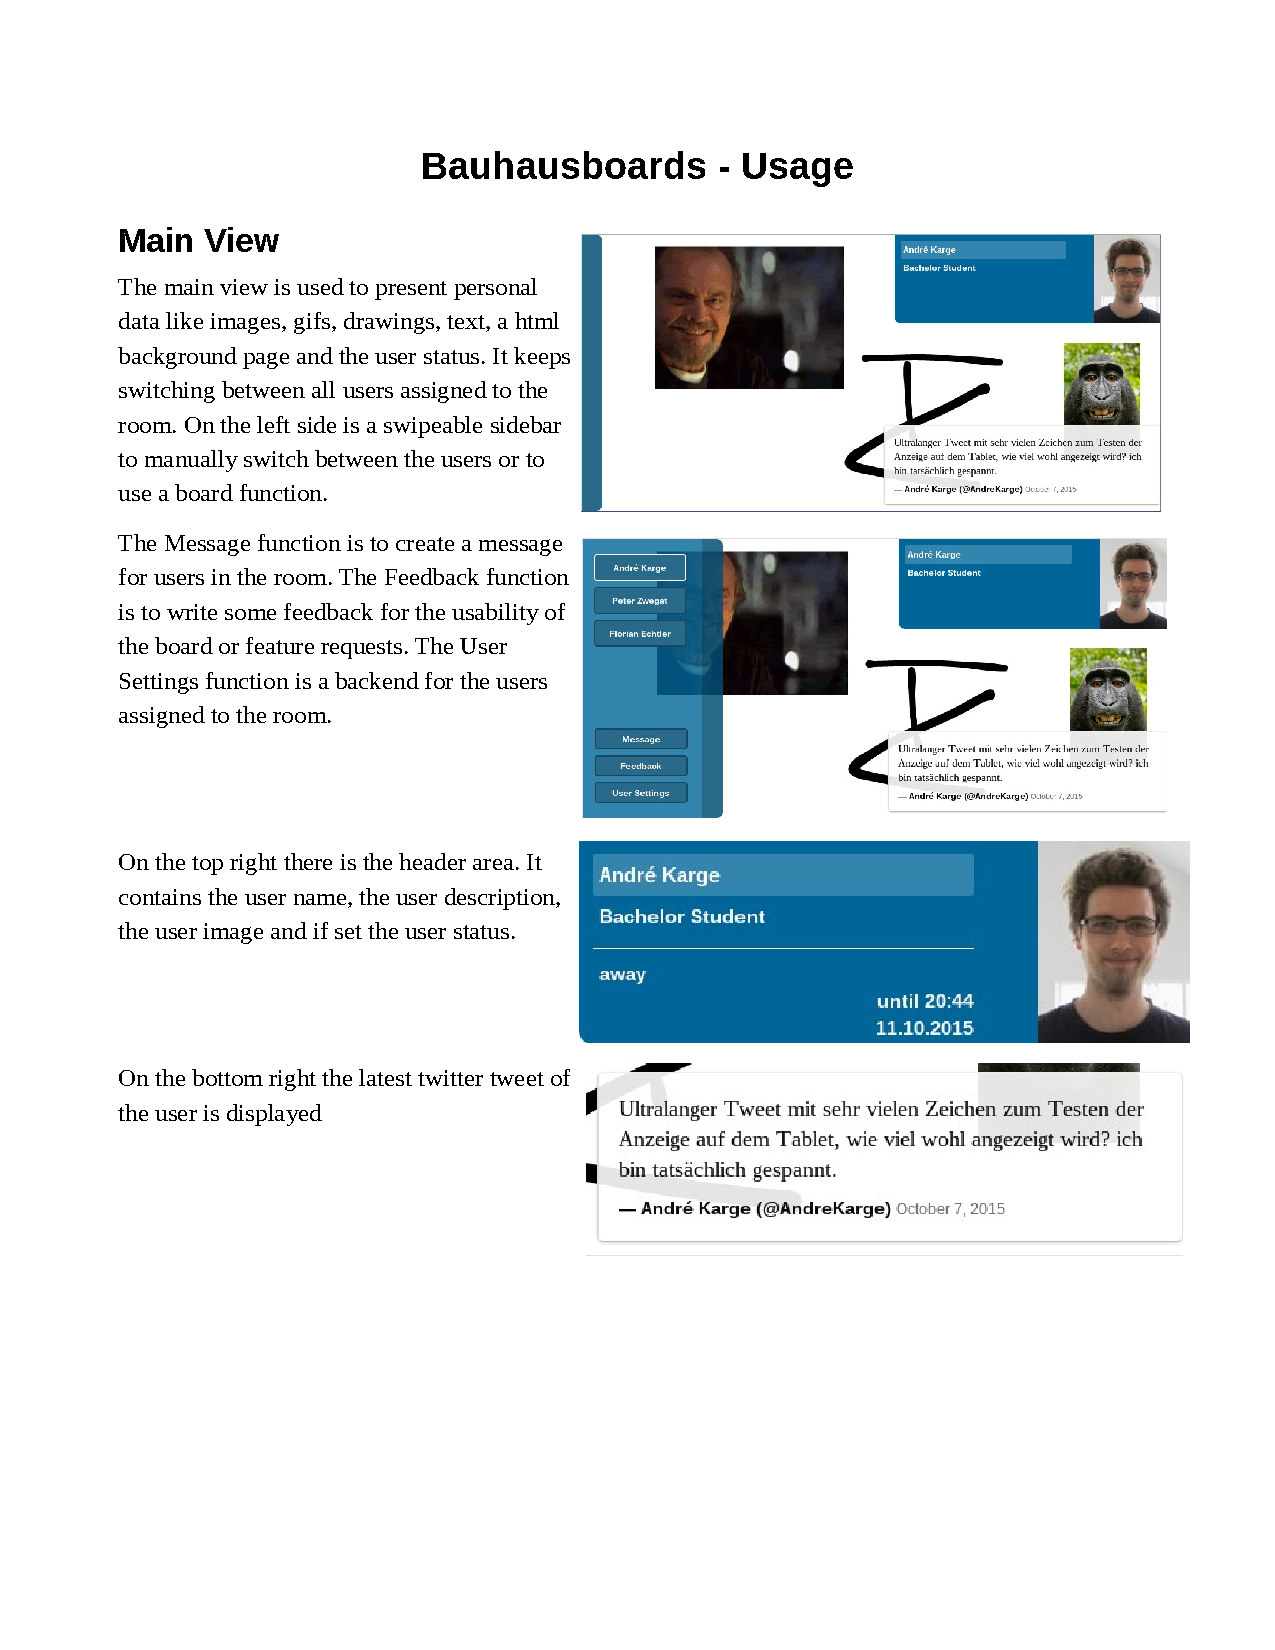
\includepdf[page=1,scale=1, pagecommand={}]{bauhausboards_how_to.pdf}
  \label{img:handbuch1}
\end{figure}
\newpage
\begin{figure}[h!]
  \centering
    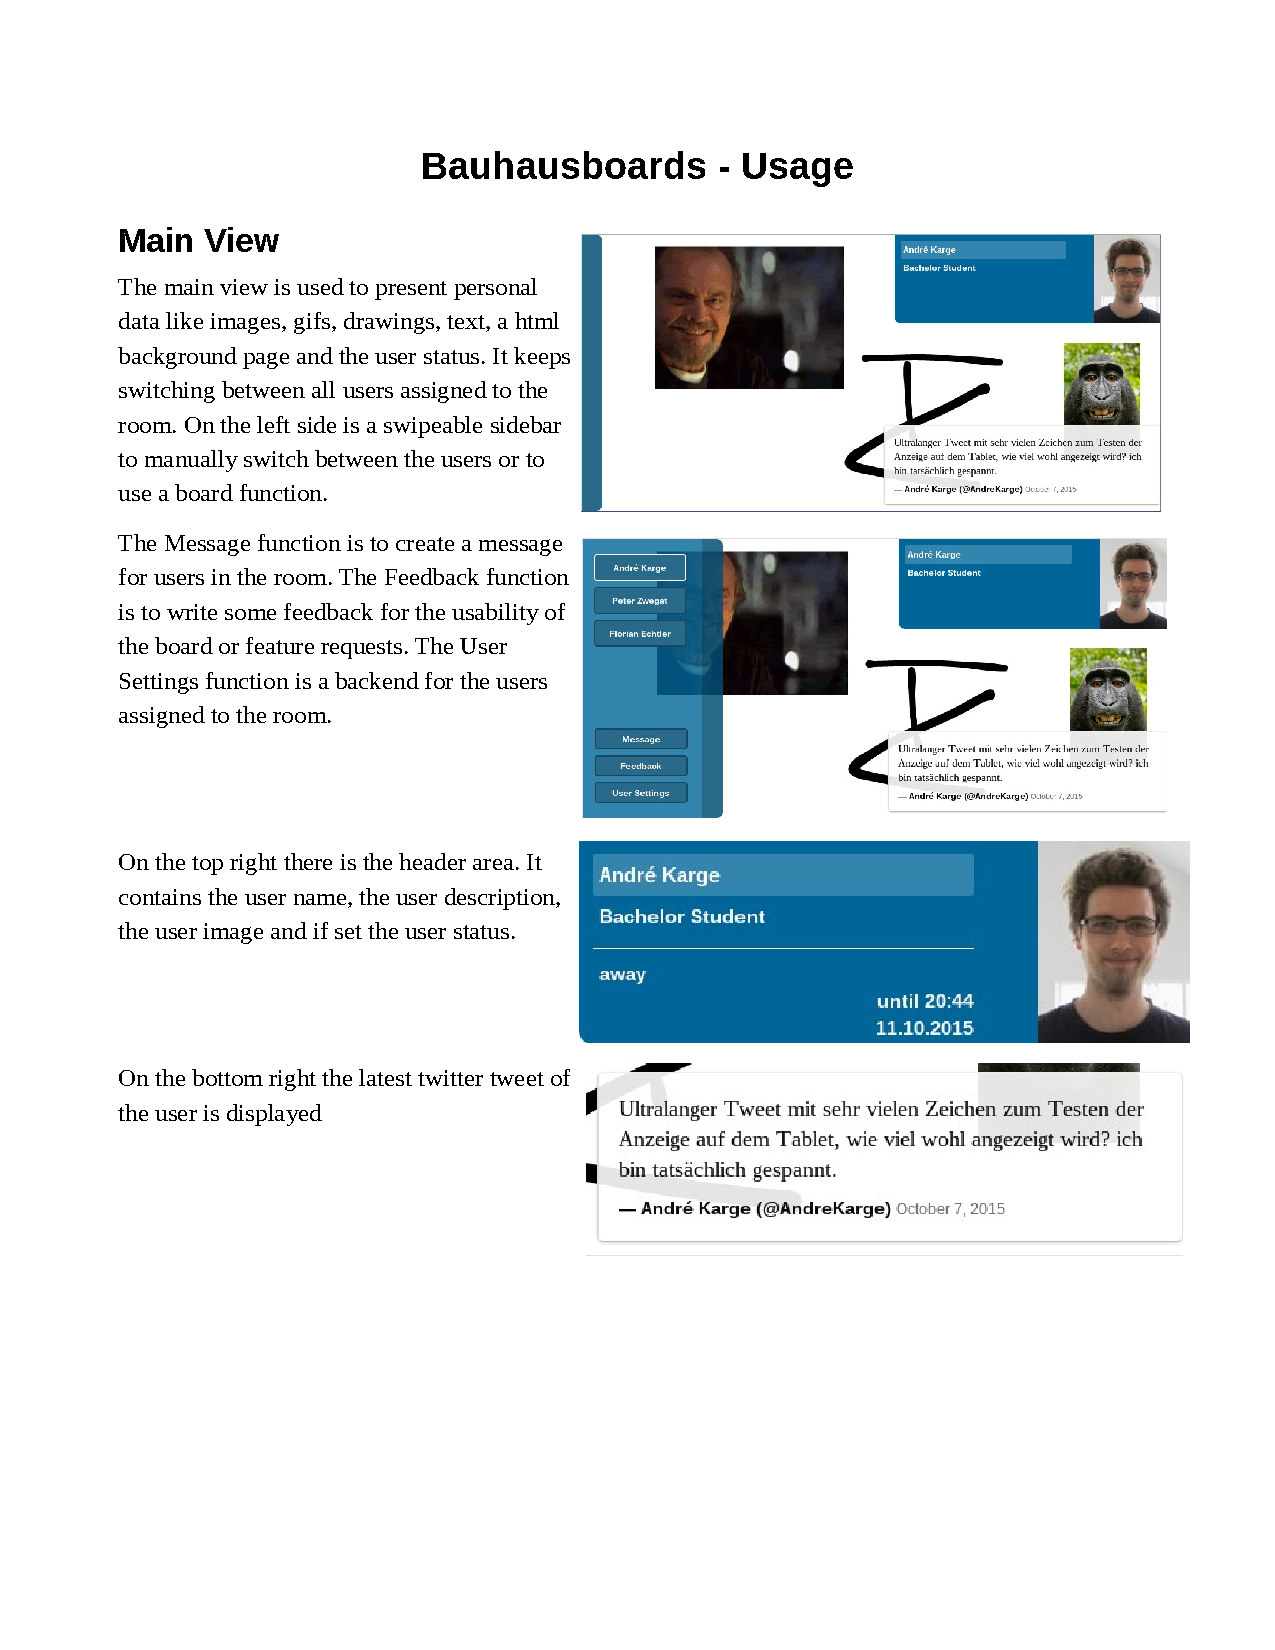
\includepdf[page=2,scale=1, pagecommand={}]{bauhausboards_how_to.pdf}
  \label{img:handbuch2}
\end{figure}
\newpage
\begin{figure}[h!]
  \centering
    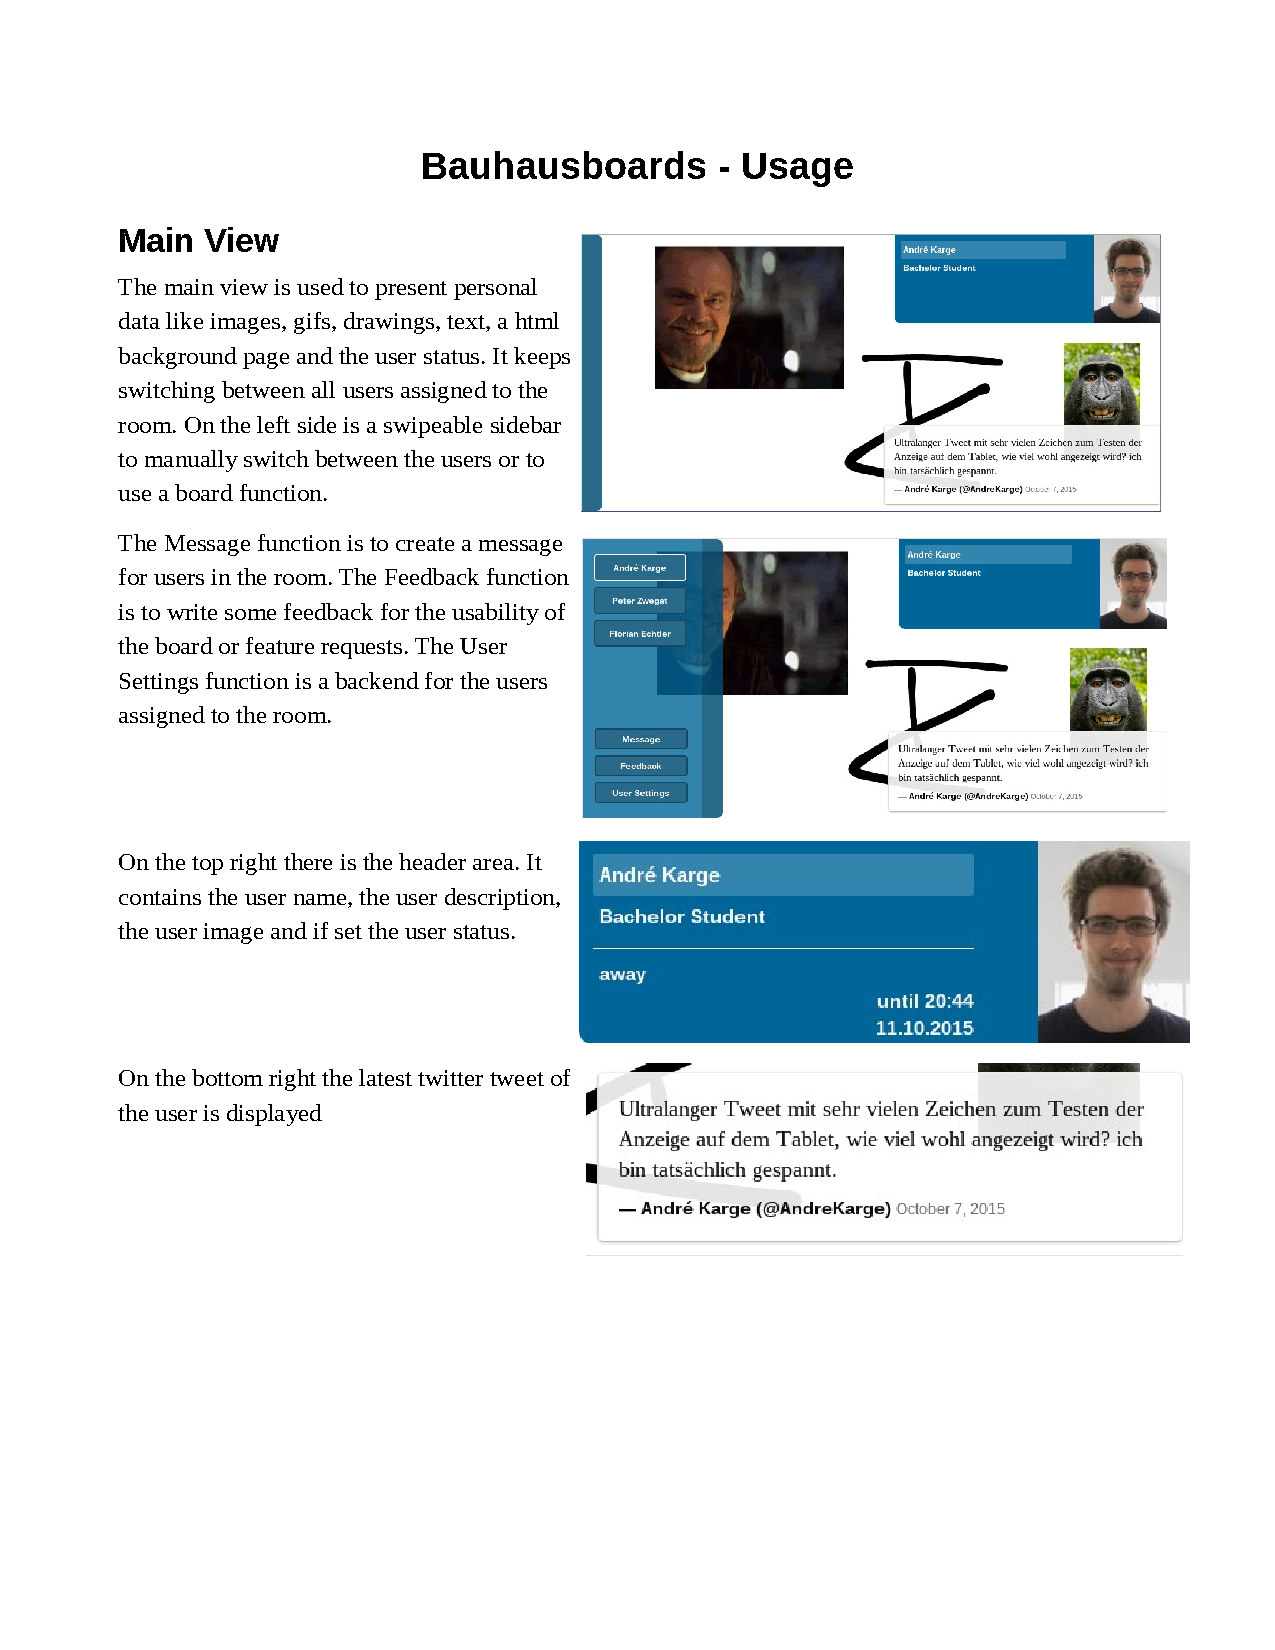
\includepdf[page=3,scale=1, pagecommand={}]{bauhausboards_how_to.pdf}
  \label{img:handbuch3}
\end{figure}
\newpage
\begin{figure}[h!]
  \centering
    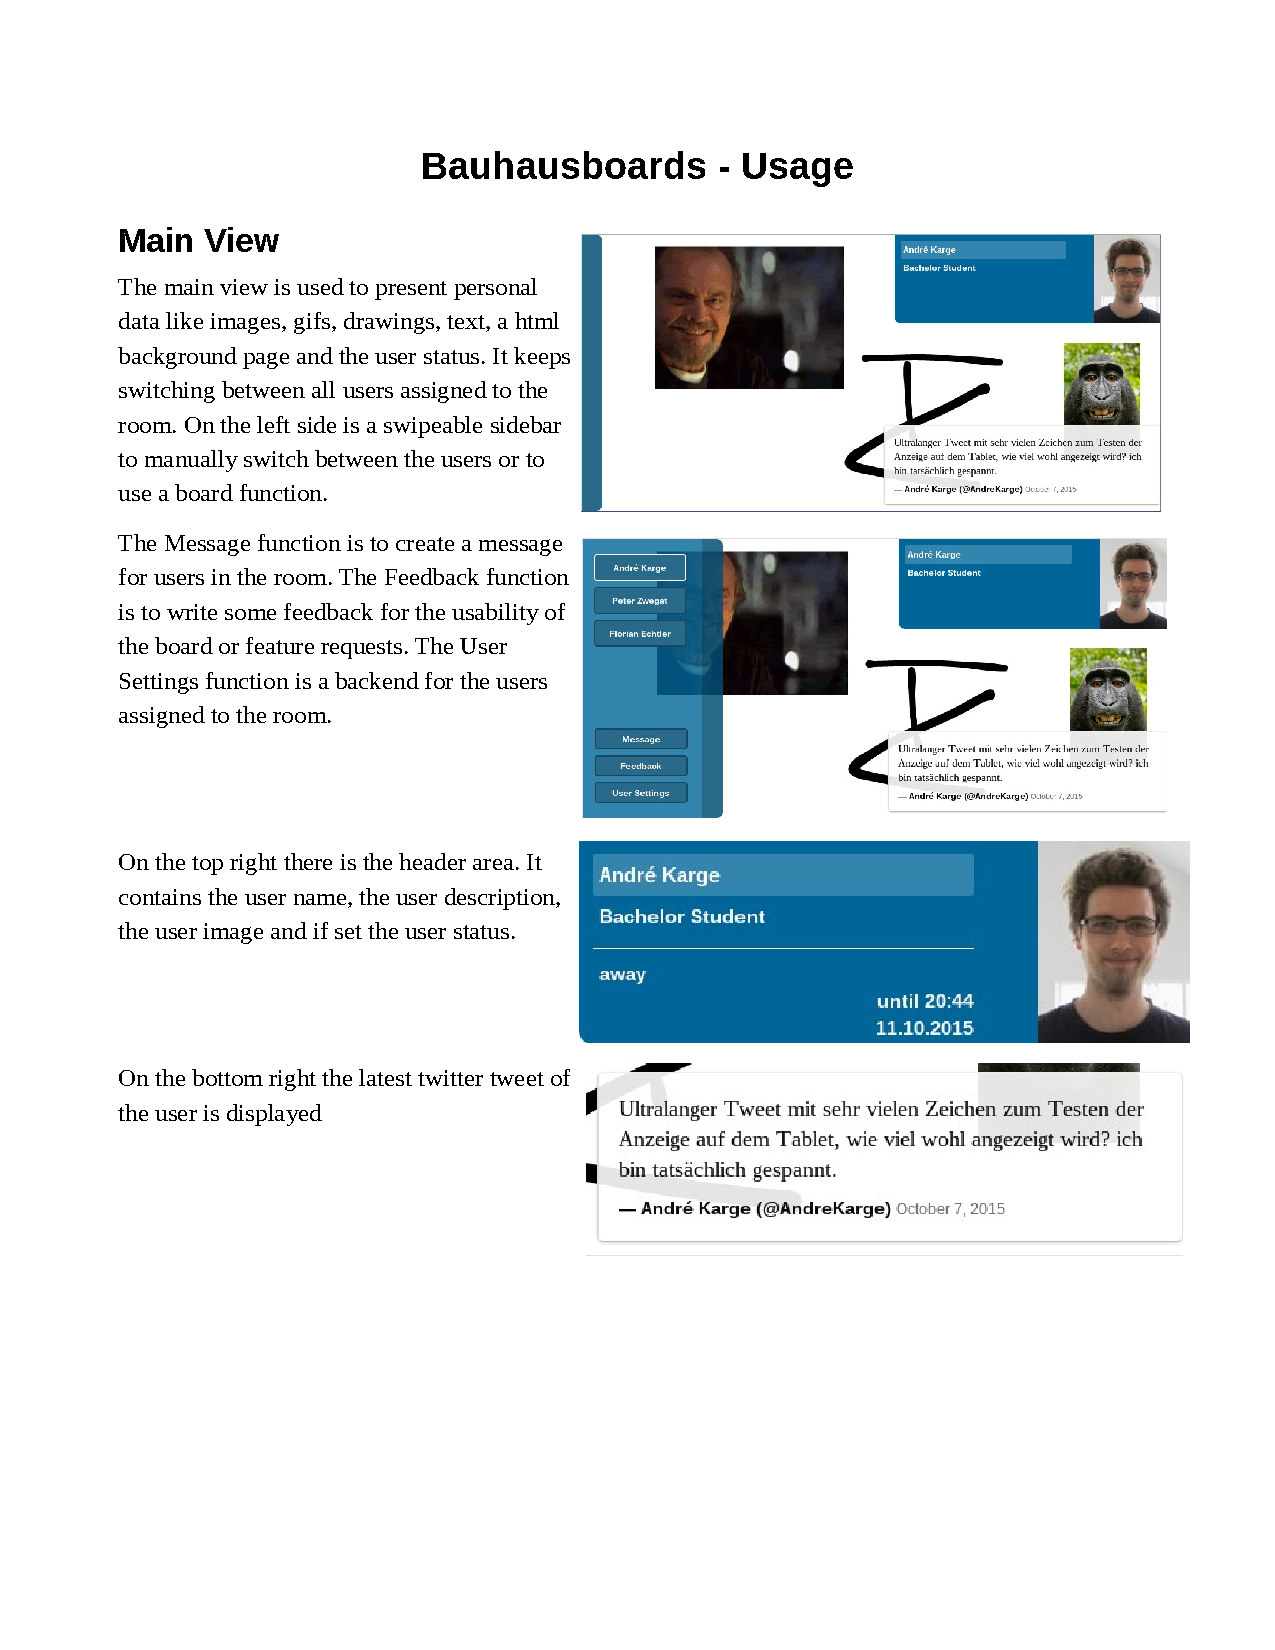
\includepdf[page=4,scale=1, pagecommand={}]{bauhausboards_how_to.pdf}
  \label{img:handbuch4}
\end{figure}
\newpage
\begin{figure}[h!]
  \centering
    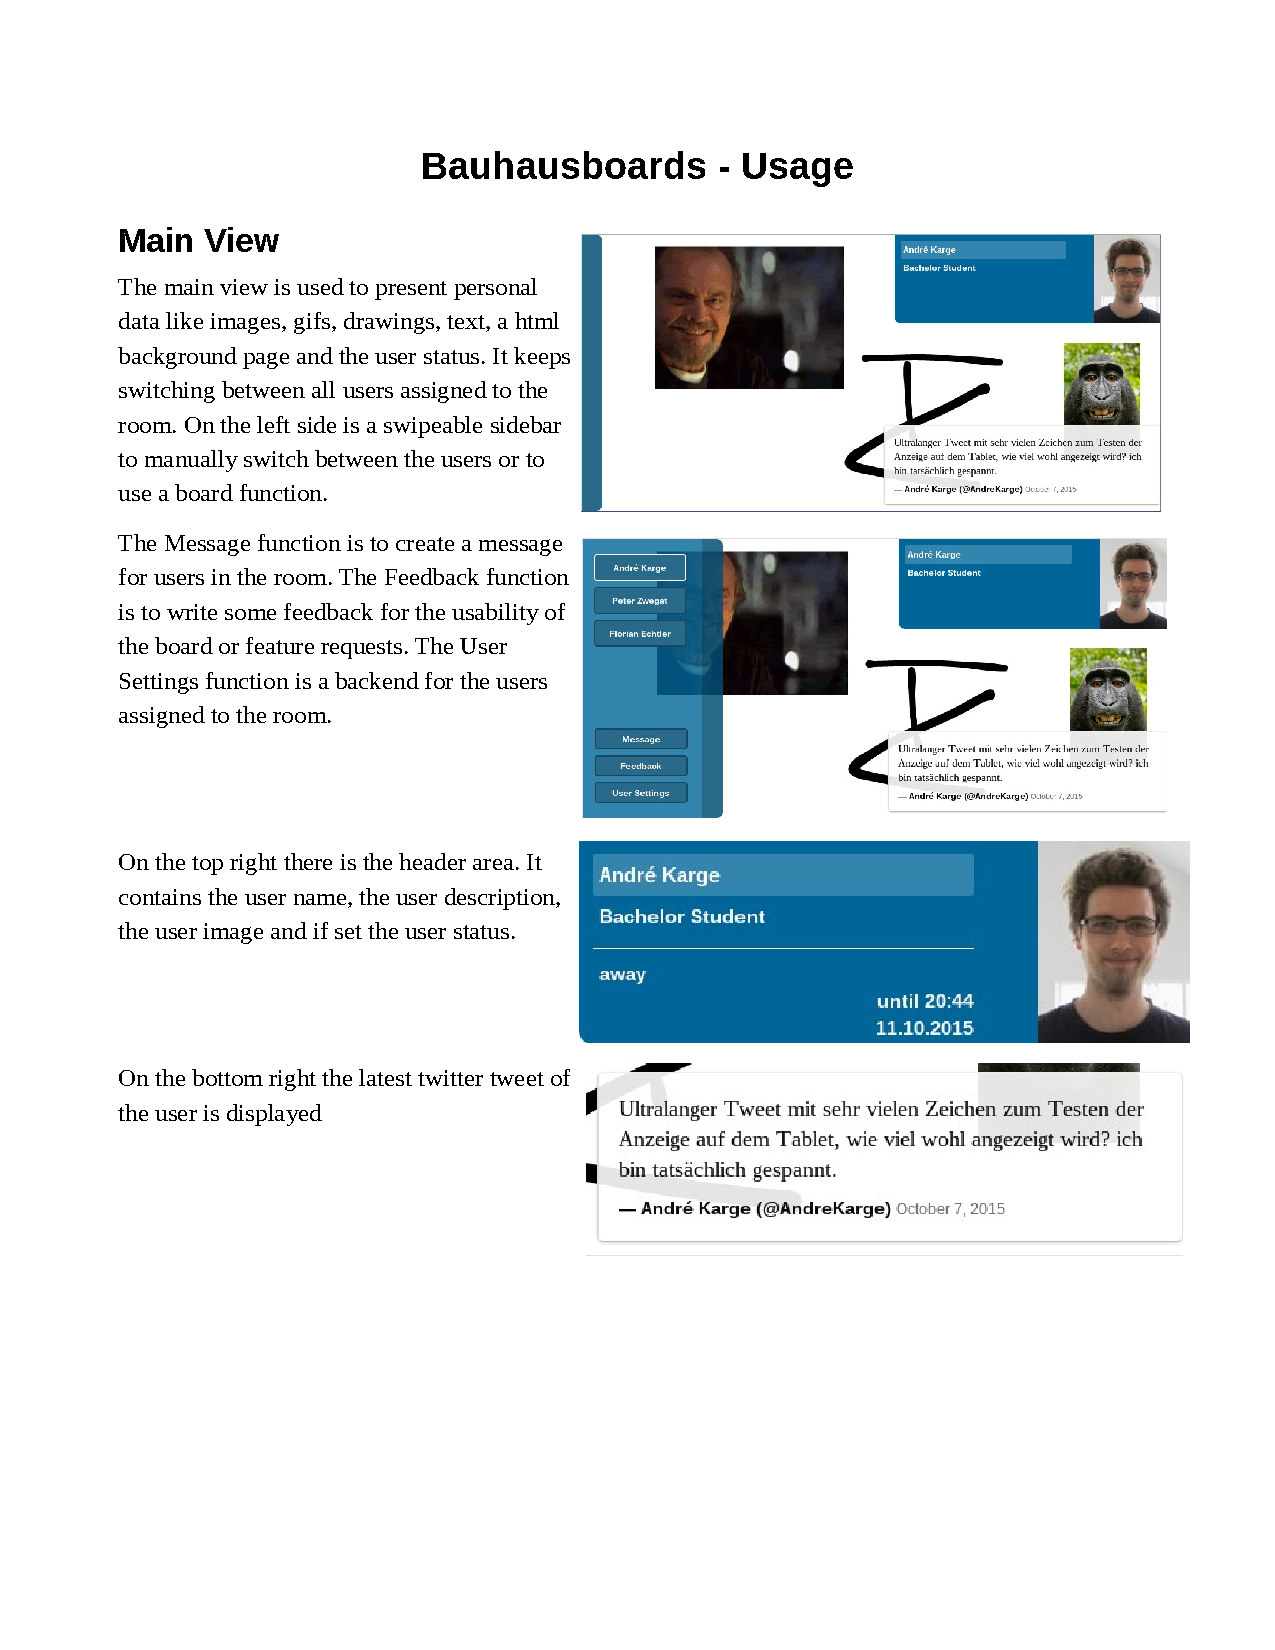
\includepdf[page=5,scale=1, pagecommand={}]{bauhausboards_how_to.pdf}
  \label{img:handbuch5}
\end{figure}
%%%%%%%%%%%%%%%%%%%%%%%%%%%%%%%%%%%%%%%%%%%%%%%%%%%%%%%%%%%%%%%%%%%%%%%%%%%%%%%%%%%%%%%%%%%%%%%%%%%%%%%%%%%%%%%%
\newpage
\markboth{Anhang - Fragestellung}{}
\begin{figure}[h!]
  \centering
    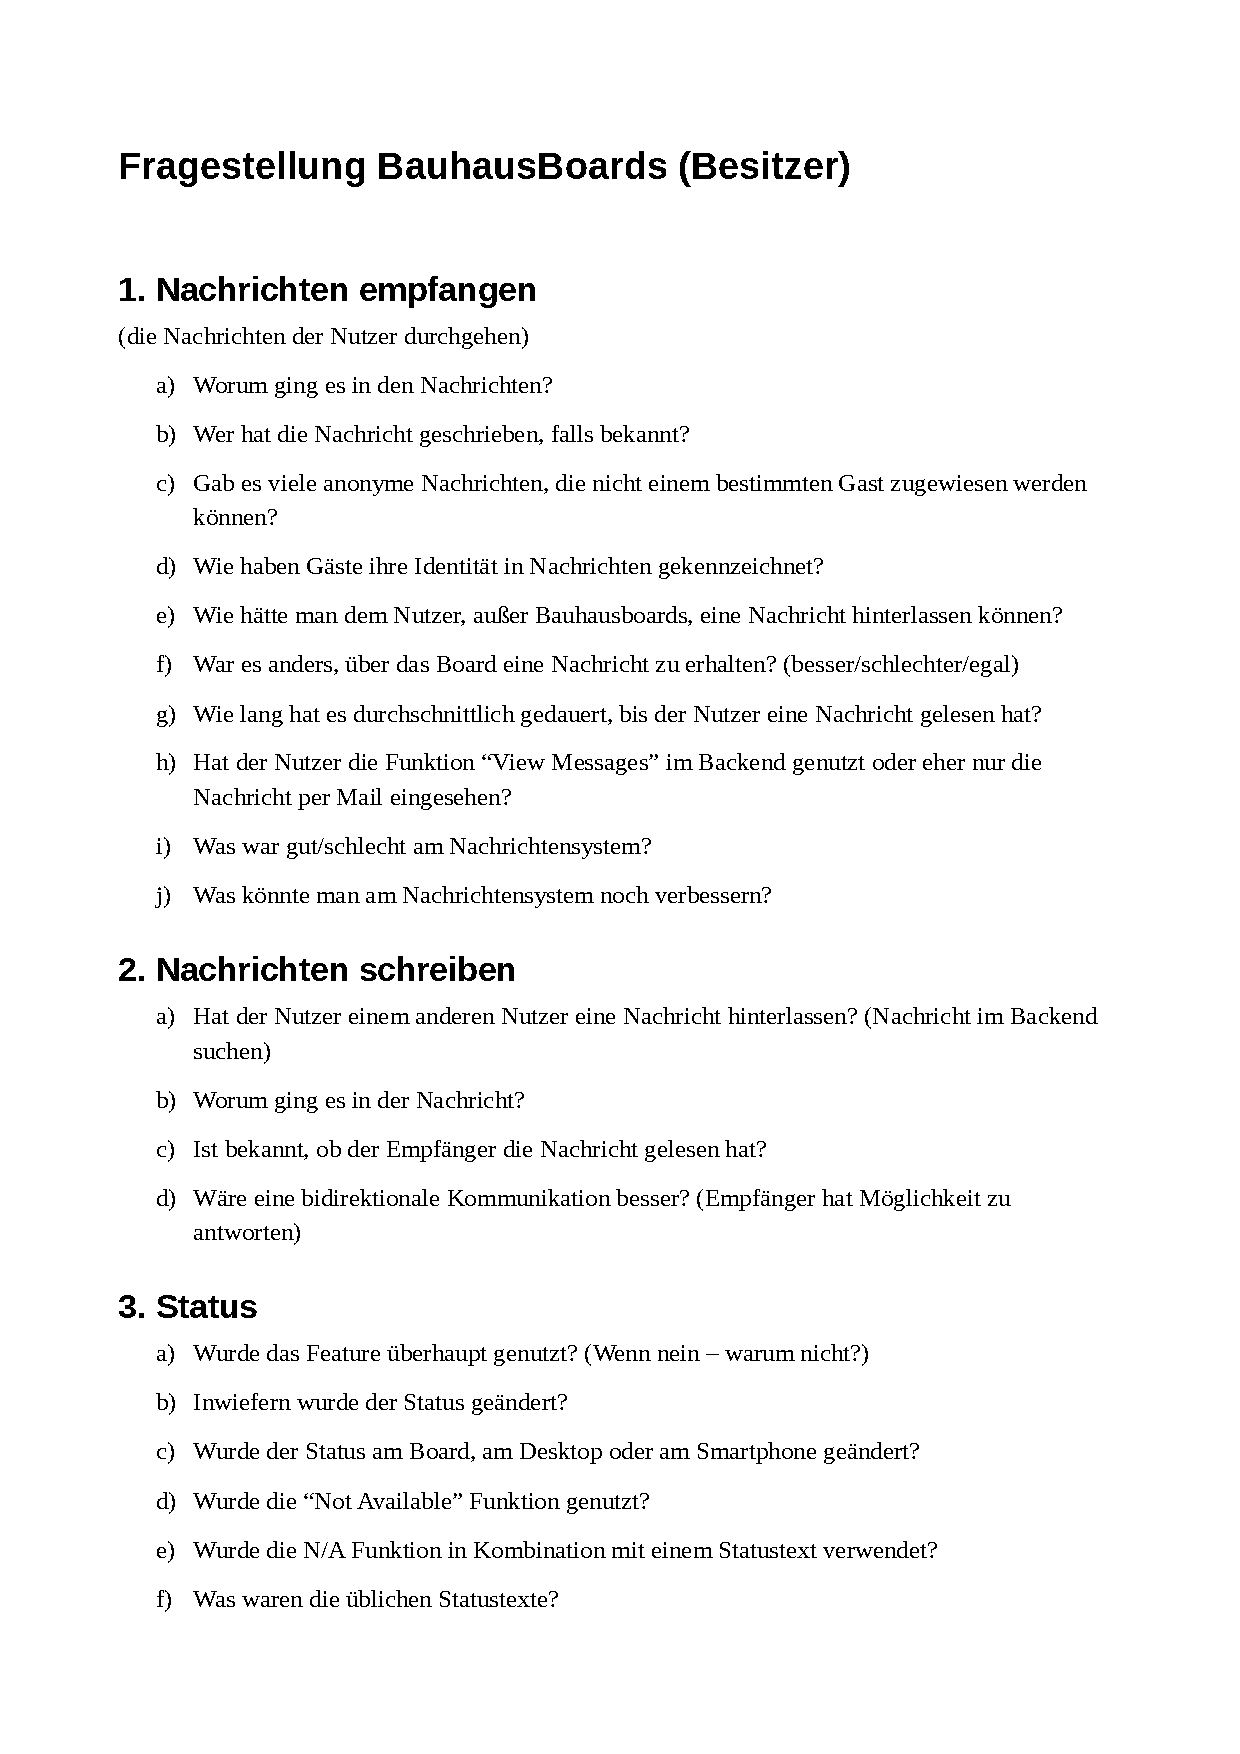
\includepdf[page=1,scale=.8, pagecommand={}]{Fragestellung_Besitzer.pdf}
  \label{img:fragestellung1}
\end{figure}
\newpage
\begin{figure}[h!]
  \centering
    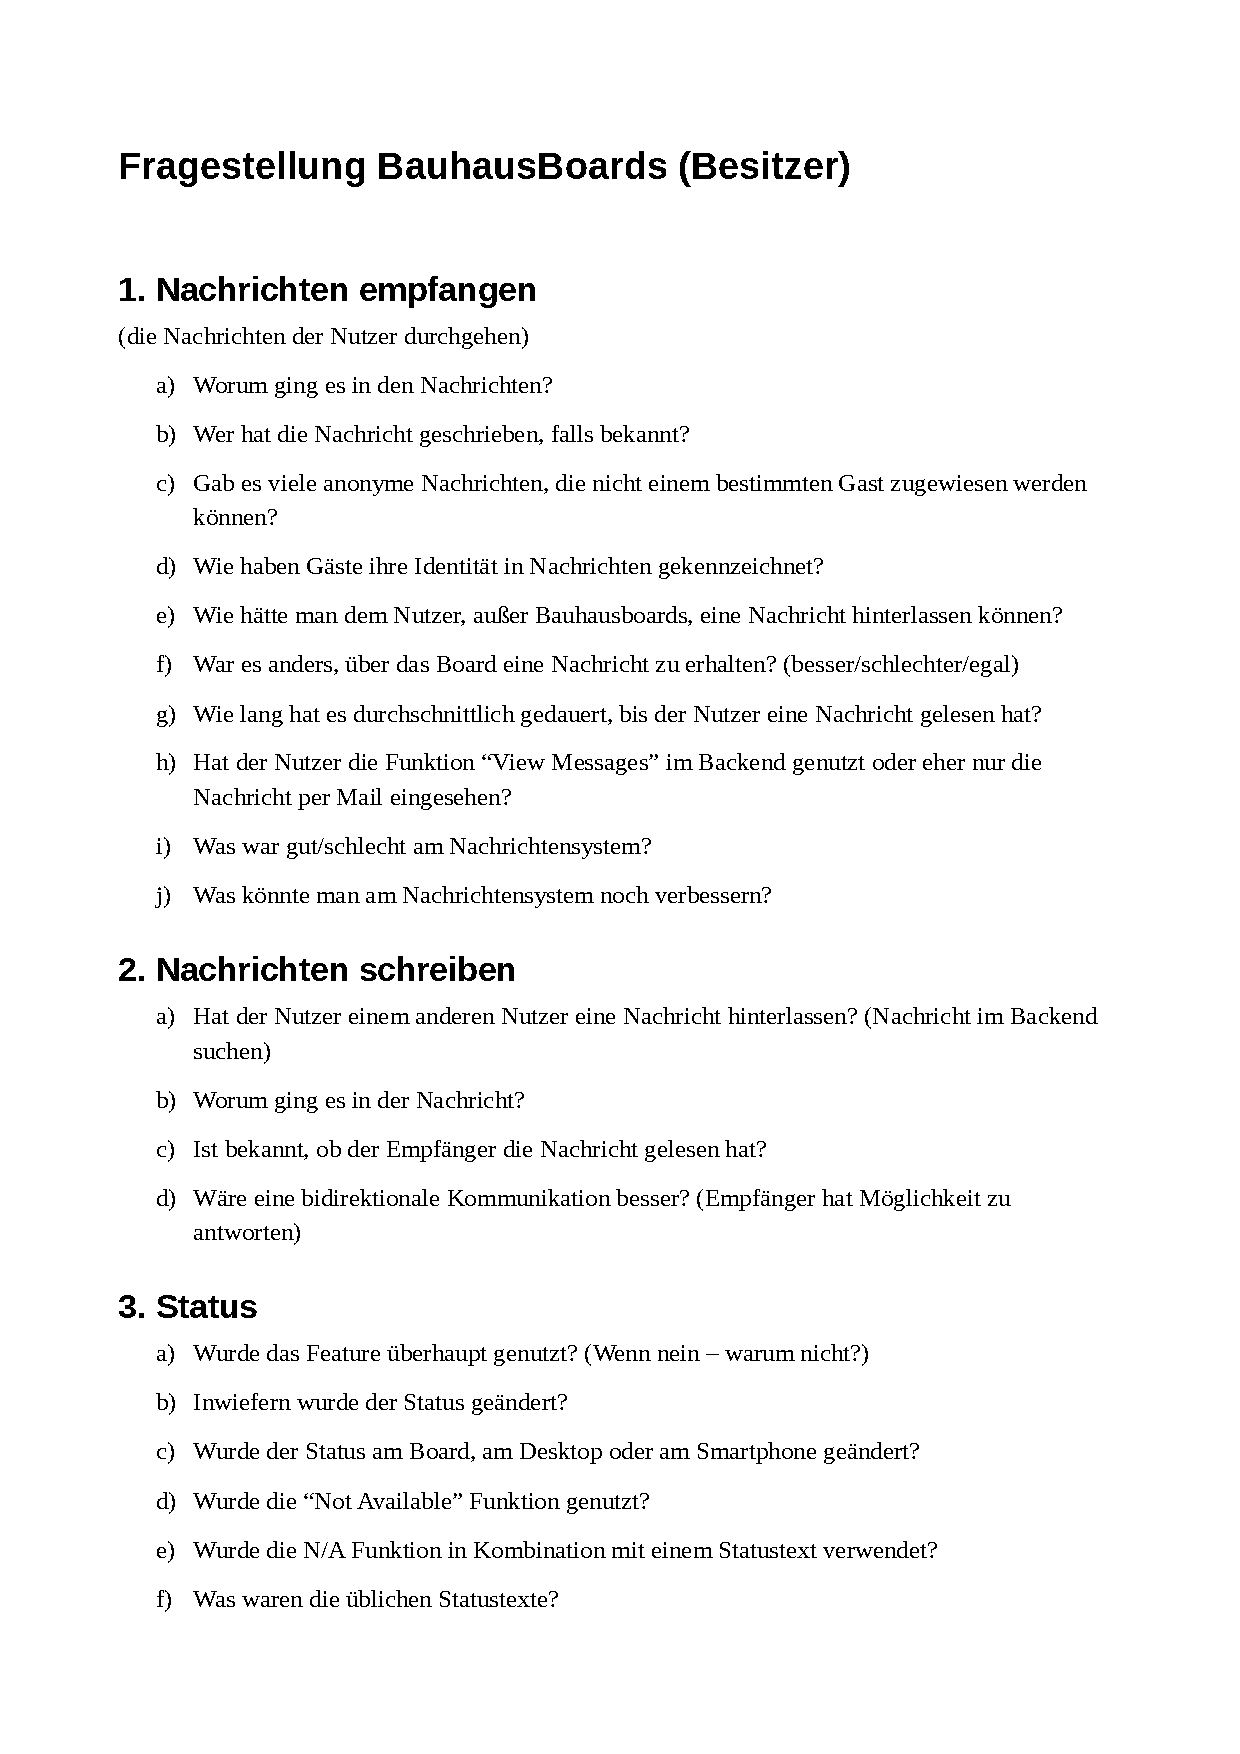
\includepdf[page=2,scale=.8, pagecommand={}]{Fragestellung_Besitzer.pdf}
  \label{img:fragestellung2}
\end{figure}
\newpage
\begin{figure}[h!]
  \centering
    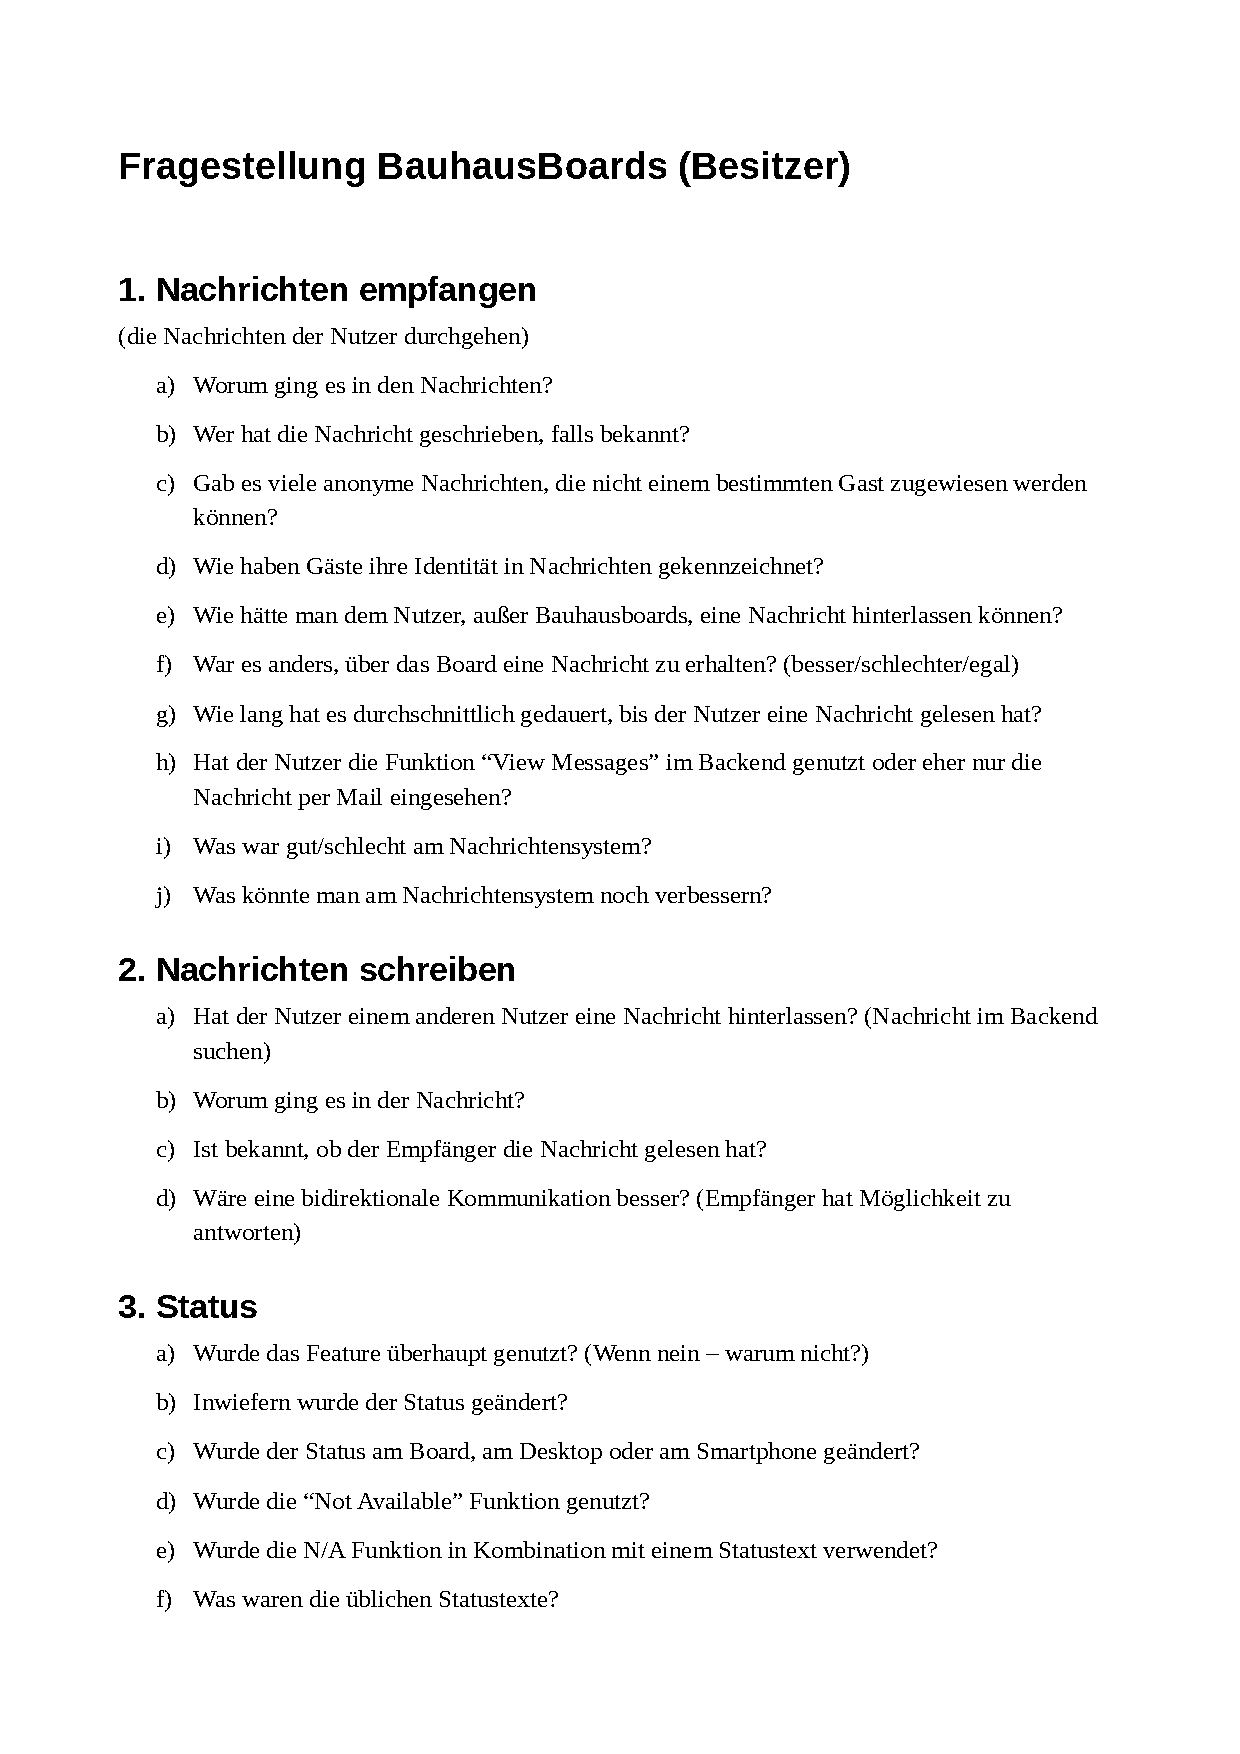
\includepdf[page=3,scale=.8, pagecommand={}]{Fragestellung_Besitzer.pdf}
  \label{img:fragestellung3}
\end{figure}